
\documentclass{standalone}
\usepackage[dvipsnames]{xcolor}
\usepackage{tikz}
\usetikzlibrary{positioning, calc, shapes, fit, backgrounds, patterns}

\begin{document}
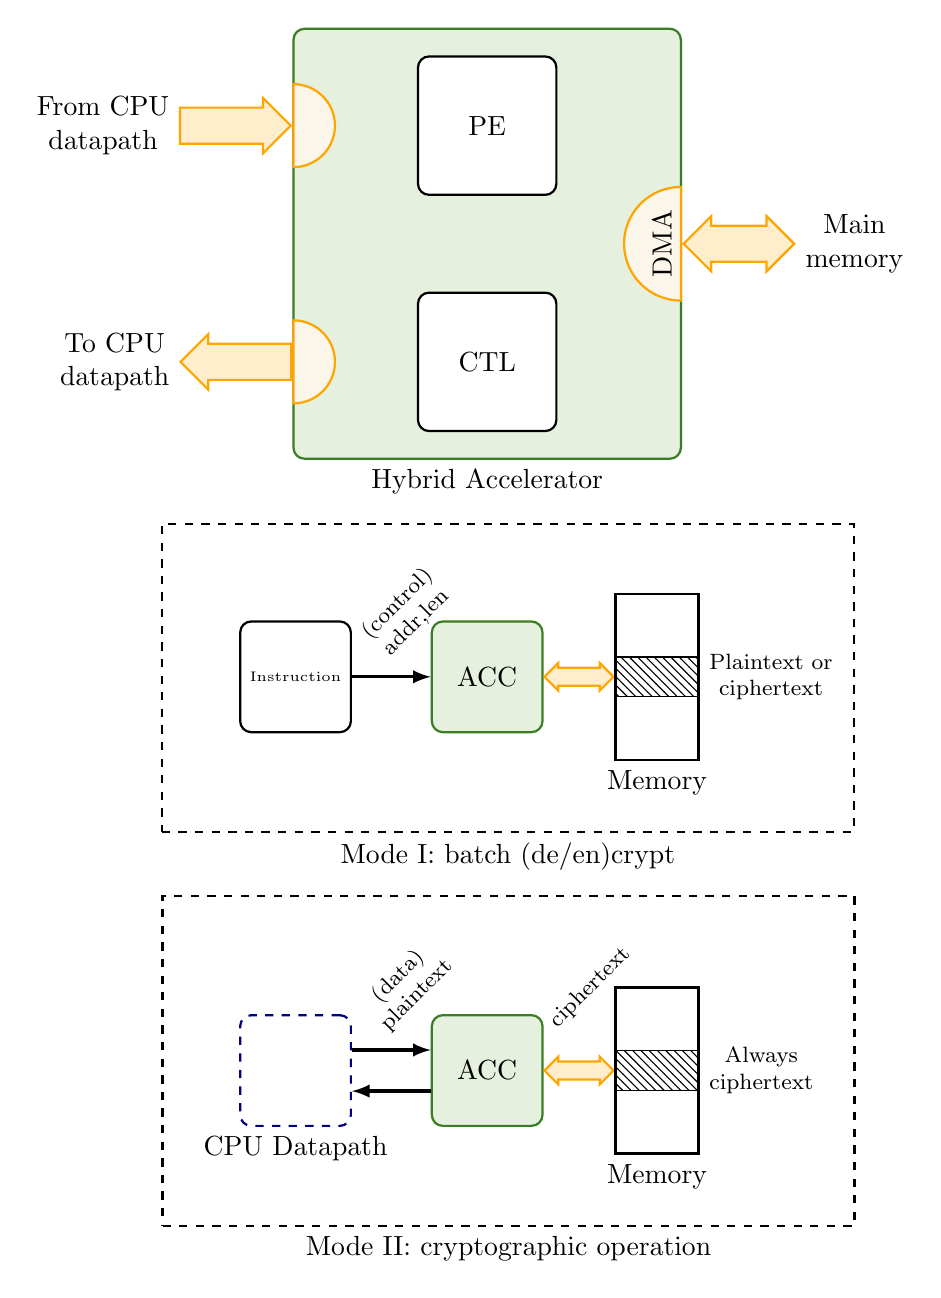
\begin{tikzpicture}
  \tikzstyle{accelement}=[rounded corners, draw, thick, minimum size=50pt, fill=white]
  \tikzstyle{port}=[semicircle, draw=Orange, fill=Goldenrod!10, anchor=south, thick]
  \tikzstyle{bibus}=[double arrow, draw=Orange, fill=Orange!20, thick,
  minimum width=20pt, double arrow head extend=2pt]
  \tikzstyle{ibus}=[single arrow, draw=Orange, fill=Orange!20, thick,
  minimum width=20pt, single arrow head extend=2pt]
  \tikzstyle{obus}=[single arrow, draw=Orange, fill=Orange!20, thick,
  minimum width=20pt, single arrow head extend=2pt, rotate=180]
  \tikzstyle{hwacc}=[rounded corners, draw=OliveGreen, fill=OliveGreen!10, thick]

  \begin{scope}[name=accstruct]
    \begin{scope}[name=acc, local bounding box=accbb]
      \node (accpe) [accelement] {PE};
      \node (accctl) at (0, -3) [accelement] {CTL};
    \end{scope}

    \begin{scope}[on background layer]
      \node (acc) [hwacc, fit=(accbb),
      minimum width=140pt, inner sep=10pt, label={270:Hybrid Accelerator}] {};
    \end{scope}

    \node (dmaport) at (acc.east) [port, minimum height=20pt, align=center,
    rotate=90] {DMA};
    \node (pathin) at (acc.west |- accpe.west) [port, rotate=270, anchor=south,
    minimum height=15pt] {};
    \node (pathout) at (acc.west |- accctl.west) [port, rotate=270, anchor=south,
    minimum height=15pt] {};

    \node (memconn) [bibus, anchor=west, minimum height=40pt, label={[align=center]0:{Main\\memory}}] at (dmaport.south) {};
    \node (fromdp) [ibus, anchor=east, minimum height=40pt, label={[align=center]180:{From CPU\\datapath}}] at (pathin.south) {};
    \node (todp) [obus, anchor=west, minimum height=40pt, label={[align=center]0:{To CPU\\datapath}}] at (pathout.south) {};
  \end{scope}

  \begin{scope}[name=op1, shift={(0, -7)}, local bounding box=mode1bb]
    \node (acc1) [hwacc, minimum size=40pt] {ACC};
    \node (inst) [draw, thick, rounded corners, left=of acc1, minimum size=40pt] {\tiny Instruction};
    \draw[-latex, very thick] (inst) -- node [anchor=south west, rotate=45, font=\footnotesize, align=center] {(control)\\addr,len} (acc1);
    \node (mconn1) at (acc1.east) [bibus, scale=0.5, anchor=west, minimum height=50pt] {};
    \node (dram1) at (mconn1.east) [draw, thick, minimum width=30pt, minimum height=60pt, anchor=west, label={270:Memory}] {};
    \draw [pattern=north west lines] (dram1.155) rectangle (dram1.335);
    \node at (dram1.east) [anchor=west, align=center, font=\footnotesize] {Plaintext or\\ciphertext};
  \end{scope}

  \node [draw,dashed, thick, fit=(mode1bb), inner sep=10pt, minimum width=250pt, label={270:Mode I: batch (de/en)crypt}, xshift=-12pt] {};

  \begin{scope}[name=op2, shift={(0, -12)}, local bounding box=mode2bb]
    \node (acc2) [hwacc, minimum size=40pt] {ACC};
    \node (dp) [draw=NavyBlue, thick, dashed, rounded corners, left=of acc2, minimum size=40pt, label={270:CPU Datapath}] {};
    \draw[-latex, very thick] (dp.20) -- node [anchor=south west, rotate=45, align=center, font=\footnotesize] {(data)\\plaintext} (dp.20 -| acc2.west);
    \draw[-latex, very thick] (dp.340 -| acc2.west) -- (dp.340);
    \node (mconn2) at (acc2.east) [bibus, scale=0.5, anchor=west, minimum height=50pt] {};
    \node (dram2) at (mconn2.east) [draw, thick, minimum width=30pt, minimum height=60pt, anchor=west, label={270:Memory}] {};
    \draw [pattern=north west lines] (dram2.155) rectangle (dram2.335);
    \node at (dram2.east) [anchor=west, align=center, font=\footnotesize] {Always\\ciphertext};
    \node at ([shift={(4pt, 30pt)}]mconn2) [align=center, rotate=45, font=\footnotesize] {ciphertext};
  \end{scope}

  \node [draw,dashed, thick, fit=(mode2bb), inner sep=10pt, minimum width=250pt,  label={270:Mode II: cryptographic operation}] {};

\end{tikzpicture}
\end{document}
